\begin{tikzpicture}[remember picture,overlay]
    \node[xshift=-0.9in,yshift=-0.9in,anchor=north east] at (current page.north east){%
    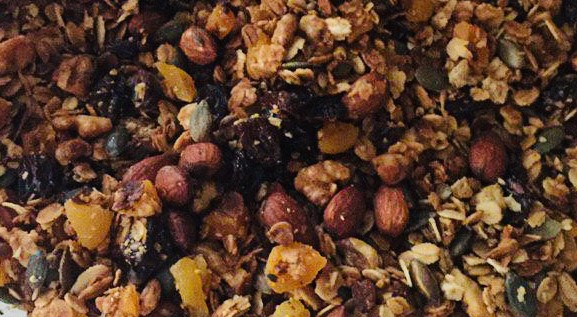
\includegraphics[width=7cm]{pic/granola}};
\end{tikzpicture}


\begin{recipe}
    [% 
        preparationtime = {\unit[15]{min}},
        bakingtime = {\unit[30]{min}}
    ]
    {Granola}
    \prerecipeoverview{\vspace{1cm}}

    \introduction{%
        There's nothing better than a quick home-made breakfast.
        Granola is a great base - add seasonal fruit, yoghurt or milk and bob's your uncle, delicious meal is ready.
    }

    \ingredients{%
        2 \nicefrac{1}{2} c. & Regular rolled oats \\
        \nicefrac{1}{2} c. & Walnuts \\
        \nicefrac{1}{2} c. & Hazelnuts \\
        \nicefrac{1}{2} c. & Sunflower seeds \\
        \nicefrac{1}{2} c. & Honey \\
        \nicefrac{1}{4} c. & Oil \\
        2 ts. & Cinnamon \\
        2 ts. & Ginger \\
        Pinch & Salt
    }

    \preparation{%
        \step Heat honey and oil slightly, just so you can mix them.
        Add spices and salt.

        \step In a big bowl, mix oats and nuts.
        Add honey/oil mixture and cover everything evenly.

        \step Transfer granola to big and flat baking tray, spread out evenly.
        \underline{Bake at  \unit[180]{\textcelcius}} 
        \underline{for 20-30 min}, mix with spatula every 5 min and keep an eye not to burn the granola!

        \step Store in an airtight jar.
    }

    \hint{%
        When the granola cooled down, you can add chopped dried fruit - eg.
        apricots and cranberry.
        You can also add some coca powder to honey - this granola will be happy when accompanied by dried cherries.
        Use different flakes (check out millet flakes or barley flakes - you can find them in polish shops certainly).
        You can also add some orange juice to honey.
        Chocolate chips, coconut flakes, etc...  There's so much room for imagination!
    }

\end{recipe}
